\documentclass[journal]{IEEEtran}

\usepackage{cite}
\usepackage{amsmath,amssymb,amsfonts}
\usepackage{graphicx}
\usepackage{textcomp}
\usepackage{xcolor}
\usepackage{listings}
\usepackage{xstring}
\usepackage{lipsum}
\usepackage{subcaption}

\newcommand{\testcase}[4]{%
	\StrRight{00#2}{2}[\paddedminor]%
	\StrRight{00#3}{2}[\paddedid]%
	\vspace{-.5em}%
	\subsection*{\textsc{FT#1\paddedminor~(TC\paddedid):} #4}%
}

\lstset{
	basicstyle=\footnotesize\ttfamily,
	breaklines=true,
	frame=single,
	captionpos=b,
	tabsize=2,
	showstringspaces=false,
	commentstyle=\color{gray},
	keywordstyle=\color{blue},
	stringstyle=\color{red},
	frame=none
}

\begin{document}
	
	\title{Testing Compliance for the Removals System}
	
	\author{Mindaugas Taujanskas}
	
	\maketitle
	
	Pursuant to the testing plan, and with the initial pre-development release completed, the following document outlines compliance with the testing criteria outlined in the aforementioned plan. Although mostly unimportant, the specifications for the testing machine are as follows:
	
	\begin{enumerate}
		\item OS: Microsoft Windows 11 Home (10.0.22631)
		\item CPU: AMD Ryzen 7 3700X (8 core) @ 3.60GHz
		\item RAM: 16GB DDR4 @ 3200MHz
		\item GPU: Radeon RX Vega 56 (8GB VRAM)
	\end{enumerate}
	
	We will run through each functional test criteria and conclude with trivial user-acceptance testing.
	
	\testcase{0}{1}{1}{Connectivity}
	As the application has very simple connection code, there is no necessity for testing it outright, since every connection parameter is configurable by the user. Rather, the testing fixture which every test requests will fail, and so will the test itself, showing a clear error.
	
	\begin{lstlisting}[language=Python]
def create_db(db_name: str, username: str = DB_USERNAME, password: str = DB_PASSWORD):
	try:
		conn = psycopg2.connect(
			database="postgres",
			user=username,
			password=password
		)
	except psycopg2.errors.OperationalError:
		g_logger.debug("failed to connect to database")
		raise
	# ...
	
	new_conn = connect_db_if_exists(db_name)
	if new_conn is None:
		raise ConnectionError(
			"Created database, but can't connect to it"
		)
	return new_conn
	\end{lstlisting}
	
	This portion of code logs and raises errors if the testing database environment is incorrectly configured, however if the production database encounters operational errors, the following code is responsible for propagating it to the user (as part of the latter specification of the test-case:)
	
	\begin{lstlisting}[language=Python]
def _register_sysexcept_handler(self) -> None:
	def handler(exctype, value, traceback) -> None:
		if QApplication.instance() is None:
			sys.__excepthook__(exctype, value, traceback)
			return
		if exctype is psycopg2.errors.OperationalError:
			QMessageBox.critical(
				None,
				"Database Error",
				"A database error occurred ..."
			)
		sys.__excepthook__(exctype, value, traceback)
	sys.excepthook = handler
	\end{lstlisting}
	
	Which shows a message-box to the user whenever the database encounters an operational error.
	
	Note that there is no unified connection function, as the testing database needs to be entirely deconstructed each test-run, which requires different procedures and privileges to the user-level application.
	
	\testcase{0}{1}{2}{Initialised schema}
	The testing database is guaranteed to be initialised on each test-run following the given code:
	
	\begin{lstlisting}[language=Python]
@pytest.fixture(scope="session")
def db_setup() -> Generator[psycopg2.extensions.connection, None, None]:
	conn = create_db(TEST_DB_NAME)
	call_goose("up")
	yield conn
	conn.close()
	call_goose("reset")
	\end{lstlisting}
	
	Which calls to the database migration management tool used for the development environment \textsc{goose}, and ensures that the latest migrations are applied and deconstructed on each test-run, so that the database is clean and up-to-date.
	
	\testcase{1}{1}{1}{Invalid credentials}
	The following tests the database-level login procedure:
	
	\begin{lstlisting}[language=Python]
def test_login_invalid_details(db_cursor):
	result = proc_login_user("a@a.com", "password")
	assert not result.success
	assert result.error.code == "INVALID_CREDENTIALS"
	\end{lstlisting}
	
	A clear error-state is shown to the user by a red underline of the entry-boxes, performed by the following:
	
	\begin{lstlisting}[language=Python]
def handle_signin(self, form: "LoginForm") -> None:
	login_data = form.get_data()
	if not form.is_valid_fields():
		return
	try:
		user = User(**login_data)
	except InvalidCredentialsError:
		form.set_all_invalid()
		return
	\end{lstlisting}
	
	By which \lstinline[language=Python]|form.is_valid_fields()| and \lstinline[language=Python]|form.set_all_invalid()| both validate and indicate fields which are incorrect to the user.
	
	\testcase{1}{1}{2}{Service-provider pending approval}
	\testcase{1}{1}{3}{Deactivated user}
	The following tests the database-level validation:
	
	\begin{lstlisting}[language=Python]
def test_login_when_pending(with_valid_user):
	email, password, _ = with_valid_user("service-provider")
	result = proc_login_user(email, password)
	assert not result.success
	assert result.error.code == "PENDING_APPROVAL"
	\end{lstlisting}
	
	And the error-state is shown by a message-box as part of the same sign-in validation procedure from FT101 (TC01:)
	
	\begin{lstlisting}[language=Python]
try:
	user = User(**login_data)
	...
except InsufficientPermissionsError as e:
	error_dialog = QMessageBox()
	error_dialog.setWindowTitle("Issue signing in")
	error_dialog.setText(
		"Your account is either not approved, ..."
	)
	error_dialog.setStandardButtons(
		QMessageBox.StandardButton.Ok
	)
	error_dialog.exec()
	form.set_all_invalid()
	return
	\end{lstlisting}
	
	Which displays a message-box and underlines all fields red. This encapsulates the criteria for both FT101 (TC02) and (TC03).
	
	\testcase{1}{2}{1}{Invalid fields}
	\testcase{1}{2}{2}{Existing email}
	Field validation is an intrinsic part of all forms in the application: when a verifiable form component is created, e.g. fulfilling FT102 (TC02):
	
	\begin{lstlisting}[language=Python]
self.email_input = LineEdit("Email", name="email")
self.email_input.register_validation_func(
	lambda email: is_valid_email(email) and exists_email(email)
)
	\end{lstlisting}
	
	Its validation function is registered at creation, and it will be automatically validated on form submission (aforementioned \lstinline[language=Python]|form.is_valid_fields|), highlighting the field as per its particular styling constraints. The test-code which ensures the database correctly recognises duplicate emails is as follows:
	
	\begin{lstlisting}[language=Python]
def test_register_duplicate_email(db_guest_cursor):
	email = random_email()
	
	first = db.proc_register_user(
		"Bob", "Builder",
		email,
		"password123",
		datetime(2000, 1, 1).date(),
		"customer"
	)
	assert first.success
	
	second = db.proc_register_user(
		"Bob", "Builder",
		email,
		"password123",
		datetime(2000, 1, 1).date(),
		"customer"
	)
	assert not second.success
	assert second.error.code == "EMAIL_EXISTS"
	\end{lstlisting}
	
	\testcase{2}{1}{1}{No DDL/DML operations}
	\testcase{2}{1}{2}{Access to exposed SQL procedures}
	DDL/DML refers to the raw retrieval/modification operations that a database user can perform on the schema, or tables. This is tested by the following:
	
	\begin{lstlisting}[language=Python]
@pytest.mark.parametrize("sql", [
	"SELECT * FROM users",
	"INSERT INTO users (first_name) VALUES ('hacker')",
	"UPDATE users SET first_name = 'bad' WHERE user_id = 1",
	"DELETE FROM users WHERE user_id = 1"
])
def test_reject_raw_table_access(db_guest_cursor, sql):
	with pytest.raises(errors.InsufficientPrivilege):
		db_guest_cursor.execute(sql)
	\end{lstlisting}

	Which is a parametrised test-case using the \texttt{app\_guest} user-role, attempting to perform DDL/DML operations, which should yield a database error as specified by the test criteria. This core logic is implemented in the permissions migration, as shown in the simplified version below:
	
	\begin{lstlisting}[language=SQL]
CREATE ROLE app_guest LOGIN PASSWORD 'app_guest';
REVOKE ALL ON ALL TABLES IN SCHEMA public FROM app_guest;
GRANT USAGE ON SCHEMA public TO app_guest;
GRANT EXECUTE ON ALL FUNCTIONS IN SCHEMA public TO app_guest;
	\end{lstlisting}
	
	The application layer should never violate this constraint natively, but the criteria must be tested to ensure integrity against malicious actors. This fulfills both criteria for FT201 (TC01) and (TC02)
	
	\testcase{2}{2}{1}{Restricted to public schema}
	
	The public schema itself is publicly exposed as FT201 (TC02) guarantees, however a \texttt{utils} schema intended for internal database usage must be restricted, as it holds the potential to expose sensitive information. This is tested in the following code:
	
	\begin{lstlisting}[language=Python]
@pytest.mark.parametrize("sql", [
	"SELECT * FROM utils.get_business_id_by_crn('12345678')",
	"SELECT * FROM utils.test_table",
])
def test_utils_schema_access_control(db_guest_cursor, sql):
	with pytest.raises(errors.InsufficientPrivilege):
		db_guest_cursor.execute(sql)
	\end{lstlisting}
	
	And implemented at the database-level in the code specified by FT201 (TC01).
	
	\testcase{3}{1}{1}{Phone number creation}
	\testcase{3}{1}{2}{Phone number retrieval}
	Phone number creation and retrieval is tested in a single function, parametrised for all subclassifications, as specified below:
	
	\begin{lstlisting}[language=Python]
@pytest.mark.parametrize("phone_type", ["home", "work"])
def test_create_phone_number(db_guest_cursor, with_valid_user, phone_type):
	email, password, result = with_valid_user("customer")
	token = result.data.token
	
	phone_result = db.proc_create_user_phone_number(
		token,
		extension="+44",
		number=f"123456789",
		phone_type=phone_type,
	)
	
	assert phone_result.success, f"Should successfully add {phone_type} phone number"
	
	fetch_result = db.proc_get_user_phone_numbers(token)
	assert fetch_result.success
	assert any(
		pn.phone_number == f"123456789"
			and pn.phone_number_type == phone_type
		for pn in fetch_result.data
	)
	\end{lstlisting}
	
	Where we are given a user account, guaranteed to be valid by FT101 (TC01), and we assign it a phone number, and then retrieve it using the provided database interface--ensuring the results are equal.
	Note that foreign key constraints guarantee attribution between a user and their phone number(s), which is out of the scope of testing as the entities are created by the SQL procedure, and as such must be tested within the SQL domain.
	
	\testcase{3}{2}{1}{Address creation}
	\testcase{3}{2}{2}{Address retrieval}
	Address creation and retrieval is tested similarly, parametrised for all its subclassifications, as specified below:
	
	\begin{lstlisting}[language=Python]
@pytest.mark.parametrize("address_type", ["home", "office", "mailing"])
def test_create_user_address(db_guest_cursor, with_valid_user, address_type):
	email, password, result = with_valid_user("customer")
	token = result.data.token
	
	address_result = db.proc_create_user_address(
		token,
		line_1=f"123 {address_type.title()} Street",
		line_2="Suite 100",
		line_3="",
		city="Bedford",
		county="Bedfordshire",
		country="United Kingdom",
		post_code="SW1A 1AA",
		address_type=address_type,
	)
	
	assert address_result.success, f"Should successfully add {address_type} address"
	
	fetch_result = db.proc_get_user_addresses(token)
	assert fetch_result.success
	assert any(
		addr.line_1 == f"123 {address_type.title()} Street"
			and addr.address_type == address_type
		for addr in fetch_result.data
	)
	\end{lstlisting}
	
	The same notes from FT301 (TC01) and (TC02) apply to address retrieval, with the addition of the fact that the country/county/city relationships are inextricably linked by look-up tables, and this relationship is tested by the following:
	
	\begin{lstlisting}[language=Python]
def test_create_invalid_address(db_guest_cursor, with_valid_user):
	email, password, result = with_valid_user("customer")
	token = result.data.token

	address_result = db.proc_create_user_address(
		token,
		line_1="123 Home Street",
		line_2="Suite 100",
		line_3="",
		city="invalid-city",
		county="Bedfordshire",
		country="United Kingdom",
		post_code="SW1A 1AA",
		address_type="home"
	)
	assert not address_result.success
	assert address_result.error.code == "INVALID_CITY"
	\end{lstlisting}
	
	\subsection{User acceptance testing}
	
	\begin{figure}[htbp]
		\centering
		\begin{subfigure}[b]{0.48\linewidth}
			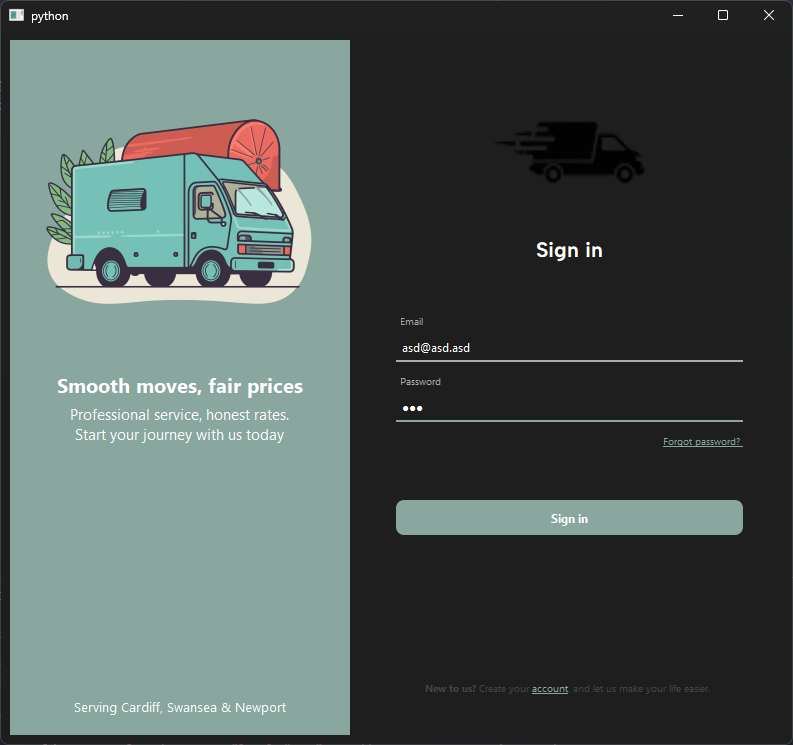
\includegraphics[width=\linewidth]{resources/uat-login-1.png}
			\caption{Login page}
		\end{subfigure}
		\hfill
		\begin{subfigure}[b]{0.48\linewidth}
			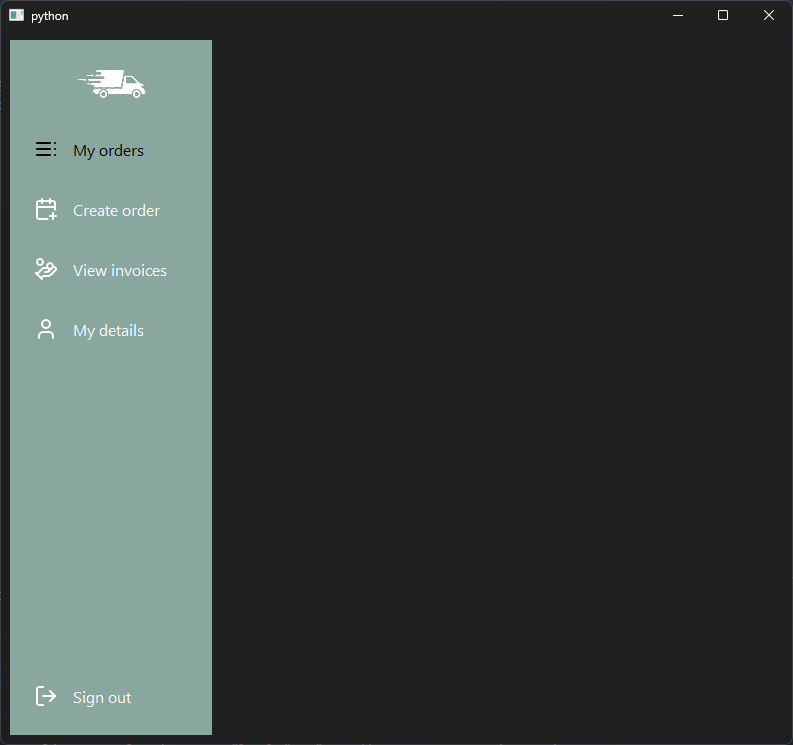
\includegraphics[width=\linewidth]{resources/uat-login-2.png}
			\caption{User dashboard after login}
		\end{subfigure}
		\caption{User login and dashboard access}
	\end{figure}
	
	After logging in successfully, the dashboard will be immediately loaded.
	
	\begin{figure}[htbp]
		\centering
		\begin{subfigure}[b]{0.48\linewidth}
			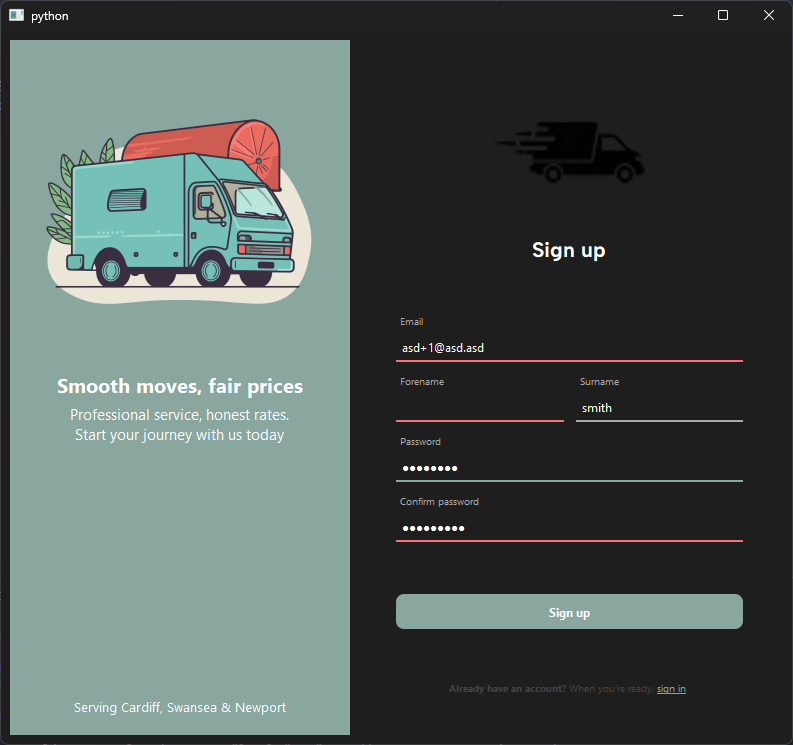
\includegraphics[width=\linewidth]{resources/uat-register.png}
			\caption{Enter registration details}
		\end{subfigure}
		\hfill
		\begin{subfigure}[b]{0.48\linewidth}
			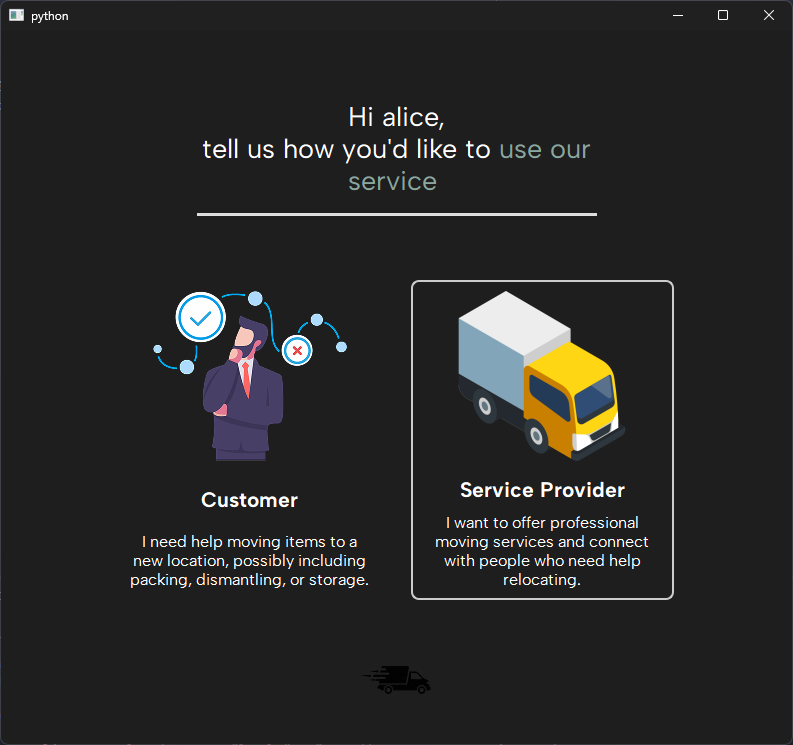
\includegraphics[width=\linewidth]{resources/uat-register-select.png}
			\caption{Select role (customer or service provider)}
		\end{subfigure}
		\caption{Initial user registration process}
	\end{figure}
	
	Fig. 2(a) demonstrates form validation with an email that corresponds to an existing one, empty required fields, and mismatching passwords. After successful submission the role selection screen is shown. Then it branches into two sections:
	
	\begin{figure}[htbp]
		\centering
		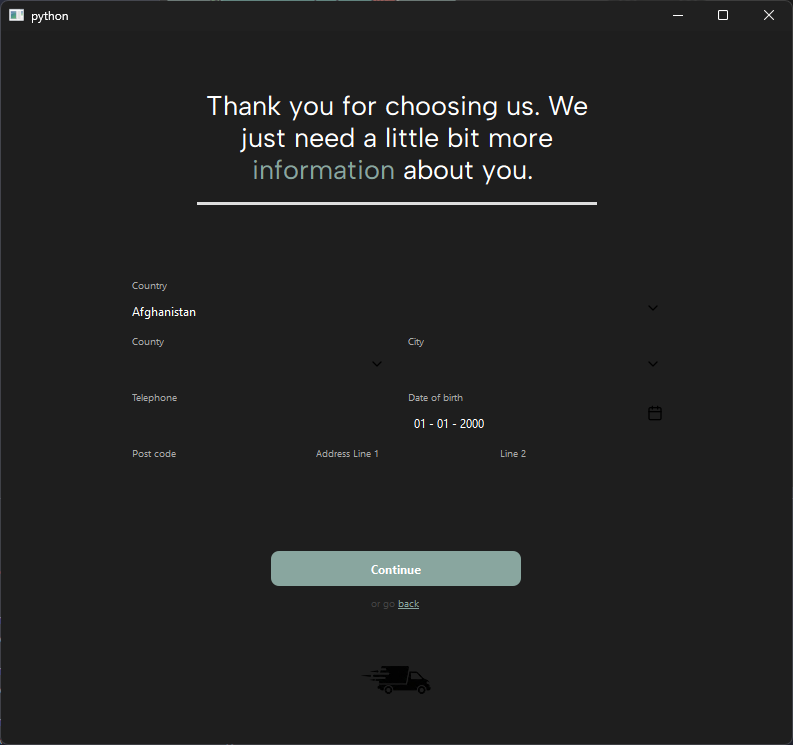
\includegraphics[width=0.6\linewidth]{resources/uat-register-customer.png}
		\caption{Customer detail submission form}
	\end{figure}
	
	After customer submission, they are taken straight to the dashboard. For service providers it is as follows:
	
	\begin{figure}[htbp]
		\centering
		\begin{subfigure}[b]{0.32\linewidth}
			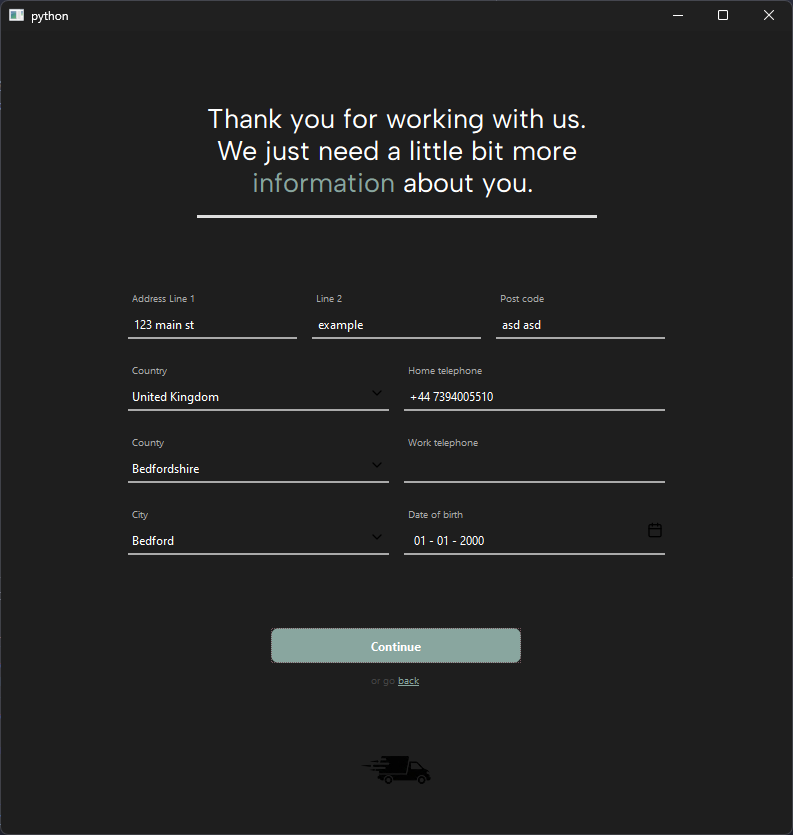
\includegraphics[width=\linewidth]{resources/uat-register-sp-1.png}
			\caption{Personal details}
		\end{subfigure}
		\hfill
		\begin{subfigure}[b]{0.32\linewidth}
			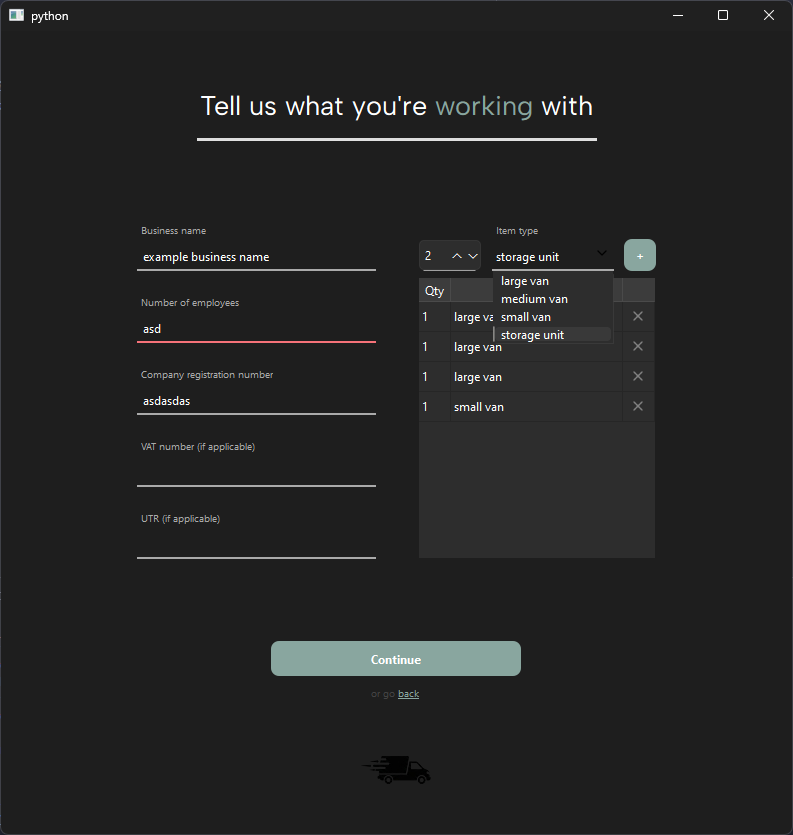
\includegraphics[width=\linewidth]{resources/uat-register-sp-2.png}
			\caption{Business details}
		\end{subfigure}
		\hfill
		\begin{subfigure}[b]{0.32\linewidth}
			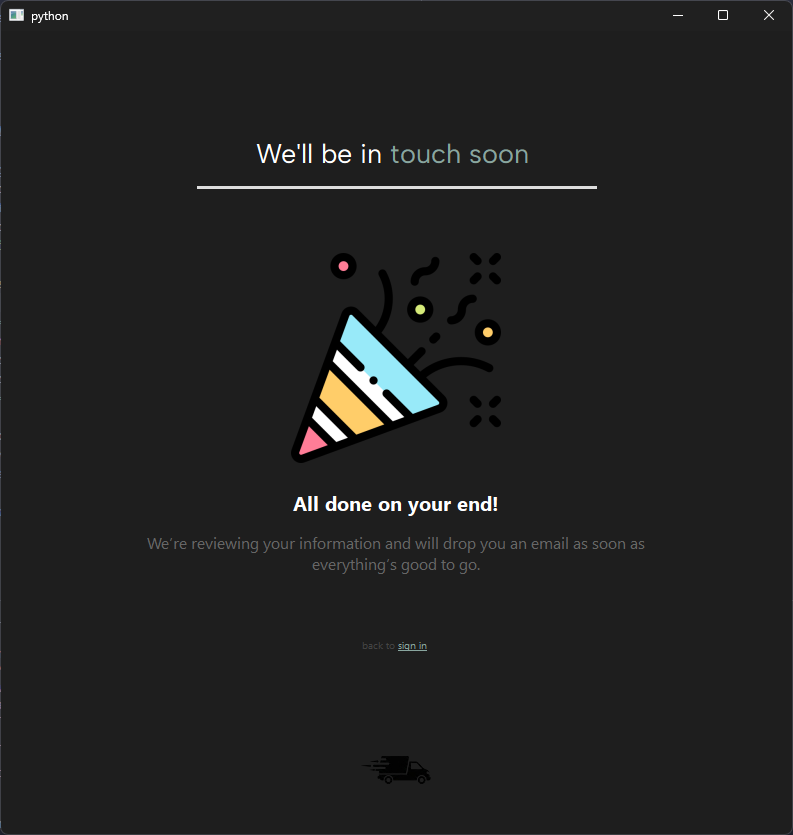
\includegraphics[width=\linewidth]{resources/uat-register-sp-3.png}
			\caption{Pending approval}
		\end{subfigure}
		\caption{Service provider registration workflow}
	\end{figure}
	
	Validation is implemented at all stages, and the service provider will be able to login after their account is approved.
\end{document}